%%%%%%%%%%%%%%%%%%%%%%%%%%%%%%%%%%%%%%%%%
% a0poster Portrait Poster
% LaTeX Template
% Version 1.0 (22/06/13)
%
% The a0poster class was created by:
% Gerlinde Kettl and Matthias Weiser (tex@kettl.de)
% 
% This template has been downloaded from:
% http://www.LaTeXTemplates.com
%
% License:
% CC BY-NC-SA 3.0 (http://creativecommons.org/licenses/by-nc-sa/3.0/)
%
%%%%%%%%%%%%%%%%%%%%%%%%%%%%%%%%%%%%%%%%%

%----------------------------------------------------------------------------------------
%	PACKAGES AND OTHER DOCUMENT CONFIGURATIONS
%----------------------------------------------------------------------------------------

\documentclass[a0,portrait]{a0poster}

\usepackage{multicol} % This is so we can have multiple columns of text side-by-side
\usepackage{csquotes} 
\columnsep=100pt % This is the amount of white space between the columns in the poster
\columnseprule=3pt % This is the thickness of the black line between the columns in the poster

\usepackage[svgnames]{xcolor} % Specify colors by their 'svgnames', for a full list of all colors available see here: http://www.latextemplates.com/svgnames-colors

\usepackage{times} % Use the times font
%\usepackage{palatino} % Uncomment to use the Palatino font

\usepackage{graphicx} % Required for including images
\graphicspath{{figures/}} % Location of the graphics files
\usepackage{booktabs} % Top and bottom rules for table
\usepackage[font=small,labelfont=bf]{caption} % Required for specifying captions to tables and figures
\usepackage{amsfonts, amsmath, amsthm, amssymb} % For math fonts, symbols and environments
\usepackage{wrapfig} % Allows wrapping text around tables and figures
\setlength{\parindent}{0pt}
\usepackage{parskip}
\setlength{\parskip}{20pt}
\usepackage[style=apa, backend=biber]{biblatex}
\addbibresource{/home/peter/home/Projects/Science/bibliography.bib}
\usepackage[compact]{titlesec}
\titlespacing{\section}{0pt}{50pt}{20pt} 

\begin{document}

%----------------------------------------------------------------------------------------
%	POSTER HEADER 
%----------------------------------------------------------------------------------------

% The header is divided into two boxes:
% The first is 75% wide and houses the title, subtitle, names, university/organization and contact information
% The second is 25% wide and houses a logo for your university/organization or a photo of you
% The widths of these boxes can be easily edited to accommodate your content as you see fit

\begin{minipage}[b]{0.75\linewidth}
\veryHuge \color{NavyBlue} \textbf{Auditory figure-ground segregation is impaired in aging and age-related hearing loss} \color{Black}\\ % Title
\huge \textbf{Péter Kristóf Velősy\footnotemark[1], Ádám Boncz\footnotemark[2], István Winkler\footnotemark[2], Brigitta Tóth\footnotemark[2]}\\[0.5cm] % Author(s)
\Large \textsuperscript{1}Department of Cognitive Science, Budapest University of Technology and Economics\\[0.4cm] %
\Large \textsuperscript{2}Institute of Cognitive Neuroscience and Psychology,
Research Centre for Natural Sciences, Budapest\\[0.4cm] % University/organization
\Large \texttt{Contact: peter@petervelosy.com}\\
\end{minipage}
%
\begin{minipage}[b]{0.25\linewidth}

\includegraphics[width=20cm]{ttk_logo.png}\\
\end{minipage}

\vspace{0cm} % A bit of extra whitespace between the header and poster content

%----------------------------------------------------------------------------------------

\begin{multicols}{2} % This is how many columns your poster will be broken into, a portrait poster is generally split into 2 columns

%----------------------------------------------------------------------------------------
%	INTRODUCTION
%----------------------------------------------------------------------------------------

\color{DarkSlateGray} % DarkSlateGray color for the rest of the content

\section*{Introduction}
\large
Listening in noisy environments is one of the fundamental capabilities of the human hearing system which is crucial for survival and for successful coping in everyday situations. While the use of hearing aids clearly improve the perception of sounds in aging users, noisy situations still present a challenge for them \autocite{Wu2013}. Amplification, therefore, is not sufficient to compensate for the loss of this ability in aging. \textcite{Teki2011} developed a novel auditory stimulus termed the Stochastic Figure-Ground (SFG). The SFG stimulus has been shown to provide a good approximation to the real-life situation of extracting a sound stream from a noisy background \autocite{Dykstra2017, Teki2013}. The successful parsing of such stimuli (figure-ground segregation - FGS) is accompanied by two ERPs: an ORN and a P600 component \autocite{Dykstra2017, Toth2016}. We presented an adapted version of the SFG stimulus \autocite{OSullivan2015} which consists of random noise made of pure tones (\textquote{ground}) and optionally an embedded set of tones consistently rising together in parallel (\textquote{figure} -- see Fig. \ref{fig:stimulus}) in a series of behavioral and electrophysiological experiments testing age related effects on the ability to detect a stream in a noisy environment.

%----------------------------------------------------------------------------------------
%	MATERIALS AND METHODS
%----------------------------------------------------------------------------------------
\section*{Materials and Methods}

\setlength{\columnsep}{60pt}
\begin{wrapfigure}{r}{0.15\textwidth}
	\begin{center}
		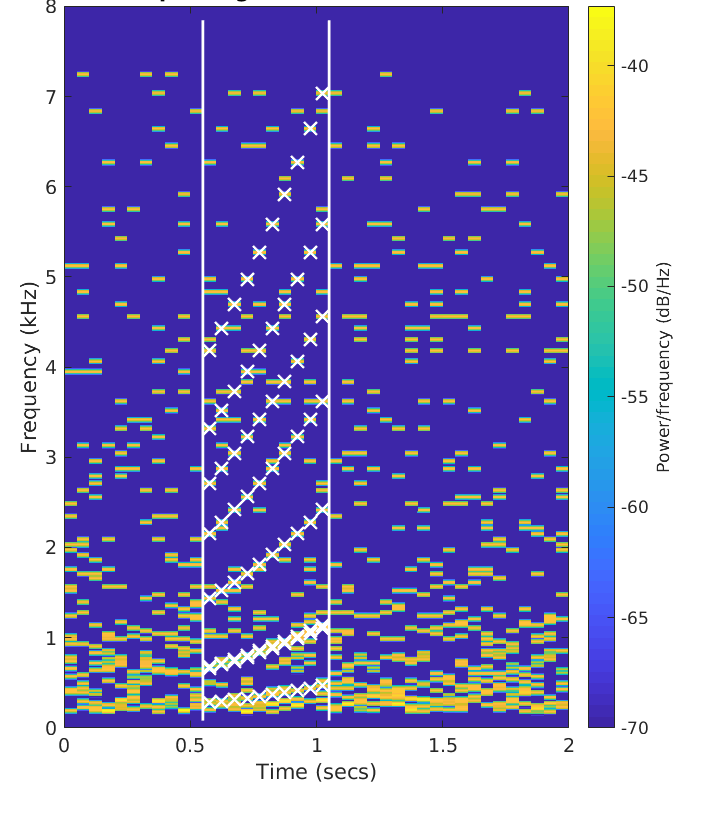
\includegraphics[width=1\linewidth]{sfg_stimulus.png}
		\captionof{figure}{\color{Green} Spectrogram of an example SFG stimulus. The x axis represents time, the y axis denotes the frequency of the tones while tone intensity is presented as a heat map (scale shown on the right). The figure consists of temporally coherent tones that are highlighted with x symbols.}
		\label{fig:stimulus}
	\end{center}
\end{wrapfigure}

\textbf{Participants}:Three groups: Young (N=21, mean age=21.2 yrs), Elderly with normal hearing (N=13, mean age=67.3 yrs), Hearing impaired elderly (N=16, 68.7 yrs)\\
\textbf{Stimuli}: SFG stimuli with or without a figure (see Fig. \ref{fig:stimulus})\\
\textbf{Pre-tests}: Audiometry examination and a digit span test was administered to evaluate hearing and general frontal functionality.\\
\textbf{Stimulus calibration}: Using an adaptive staircase method, the number of consistently rising parallel tones (\textquote{figure coherence}) was set individually for each participant such that they performed the figure detection task separately at 60\% and 80\% accuracy (\textquote{low-SNR} and \textquote{high-SNR} condition, respectively). No other parameter was adjusted.

\textbf{Task}: Participants listened to a random series of high and low-SNR SFG stimuli (.5 probability, each), each either containing a figure or not (.5 probability, each). They were instructed to judge whether the figure was present or not. \\
\textbf{Recorded data}: Behavioral measures (accuracy, reaction time) + EEG
\section*{Behavioral results}

	 \textbf{Stimulus calibration successfully compensated for individual performance differences.} While we found significantly higher accuracy (d') and lower reaction times in the high- relative to the low-SNR condition, there was no significant group difference. Thus, both the individual adjustments and the SNR manipulation were successful.
	
	 \textbf{Hearing impairment has an effect on FGS ability} The figure coherence values needed to reach the same performance were significantly higher for the hearing impaired elderly than for the other two groups.
	 
	 \begin{center}\vspace{0cm}
	 	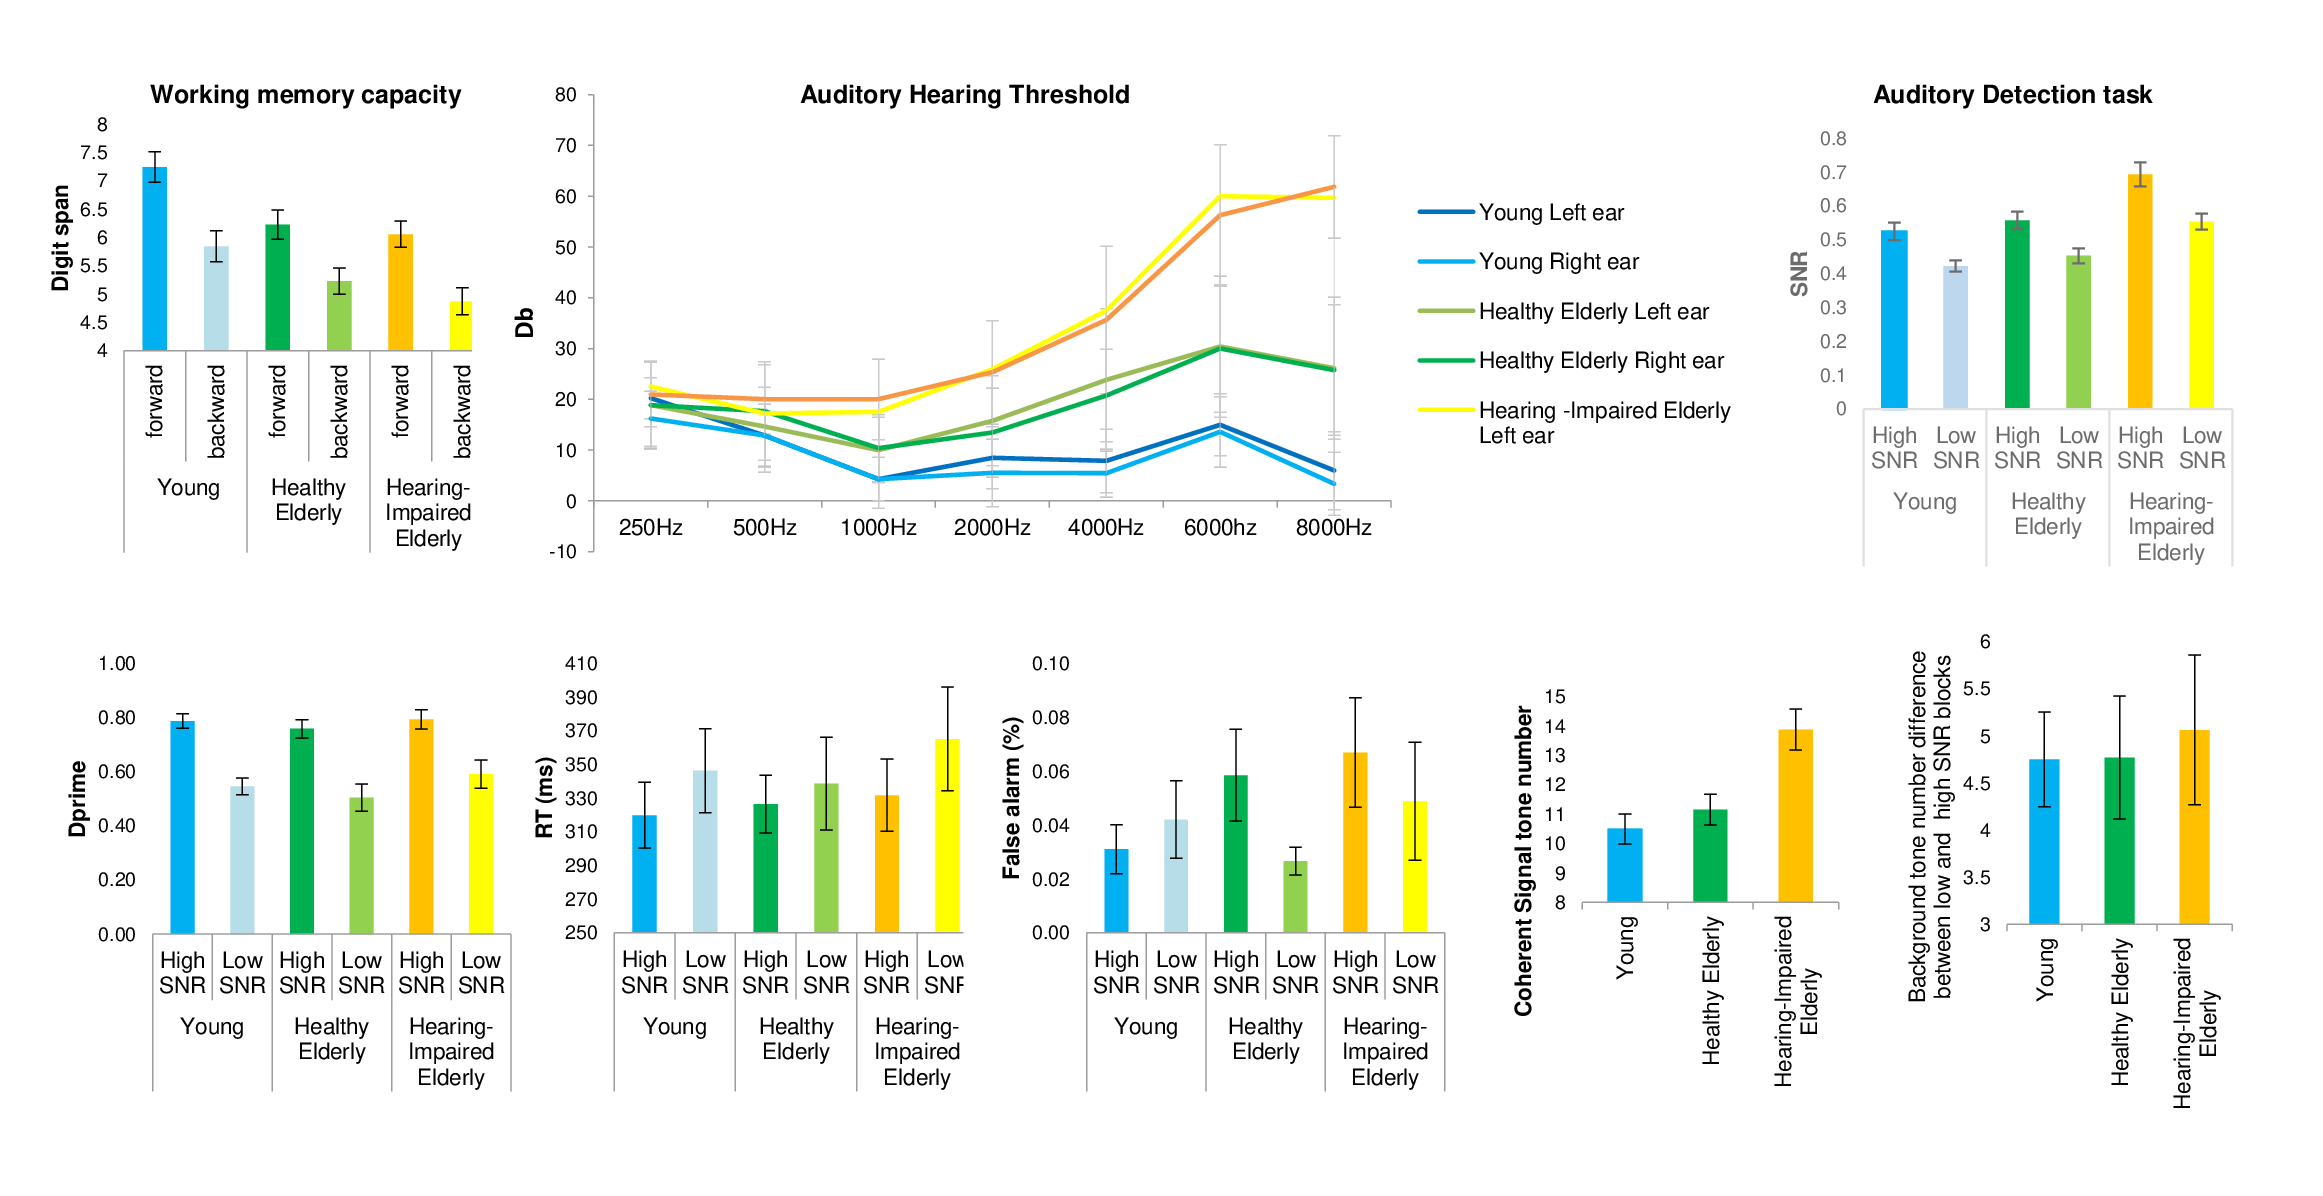
\includegraphics[width=0.95\linewidth]{Fig_behav.png}
	 	\captionof{figure}{\color{Green} Behavioral results}
	 \end{center}\vspace{0cm}
 
 %\vfill\null
 %\columnbreak
 
 \section*{EEG results}
	
	 \textbf{The ORN amplitude showed an effect of SNR but no effect of aging or hearing impairment.} The main effect of SNR was significant due to a higher ORN for high- than low-SNR trials.
	
	 \textbf{The P600 amplitude showed an effect of age but no effect or SNR or hearing impairment.} The P600 response showed higher amplitude in young subjects than in elderly subjects with or without hearing impairment. The two elderly groups did not significantly differ from each other.
	
	\textbf{According to source localization, the ORN was elicited in left Heschl's gyrus, STG, IFG, MFG, MTG, SMG whereas the P600 component was strongest in the anterior and posterior cingular cortices and in posterior brain regions (lingual and pericalcarine gyri)}.

\begin{center}\vspace{0cm}
	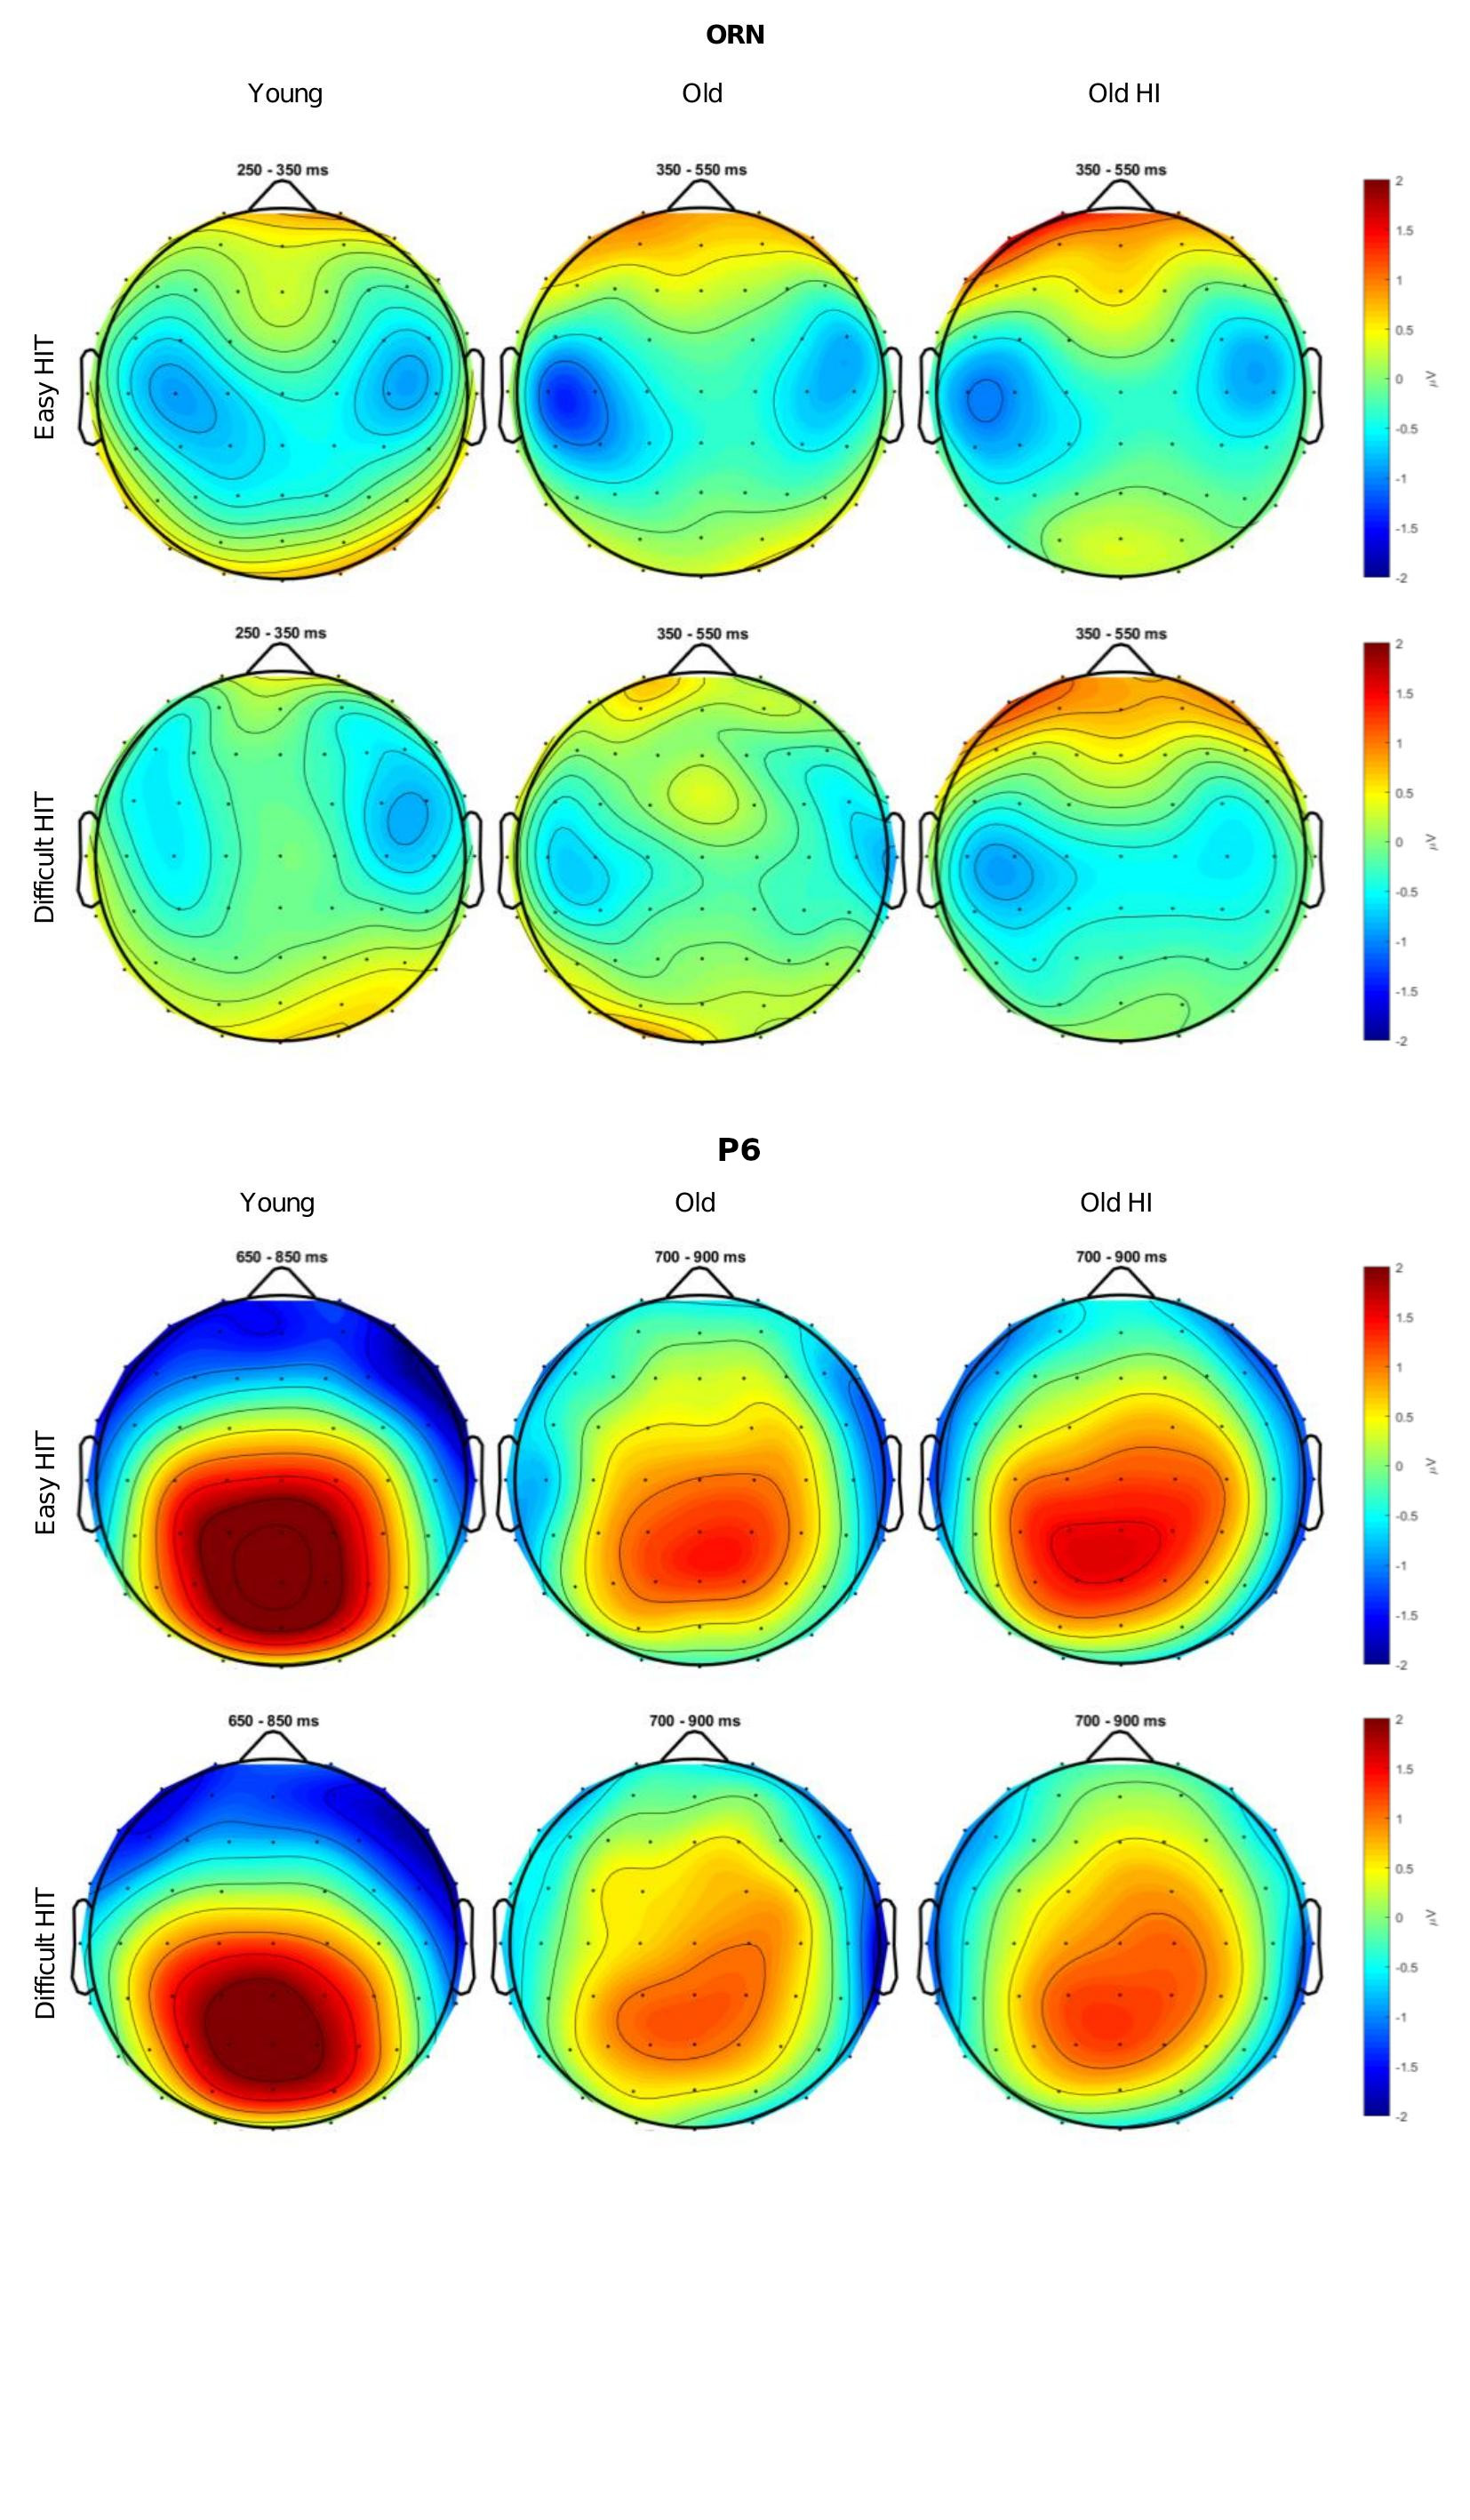
\includegraphics[width=0.35\linewidth]{ORN_P4_4x3.jpg}
	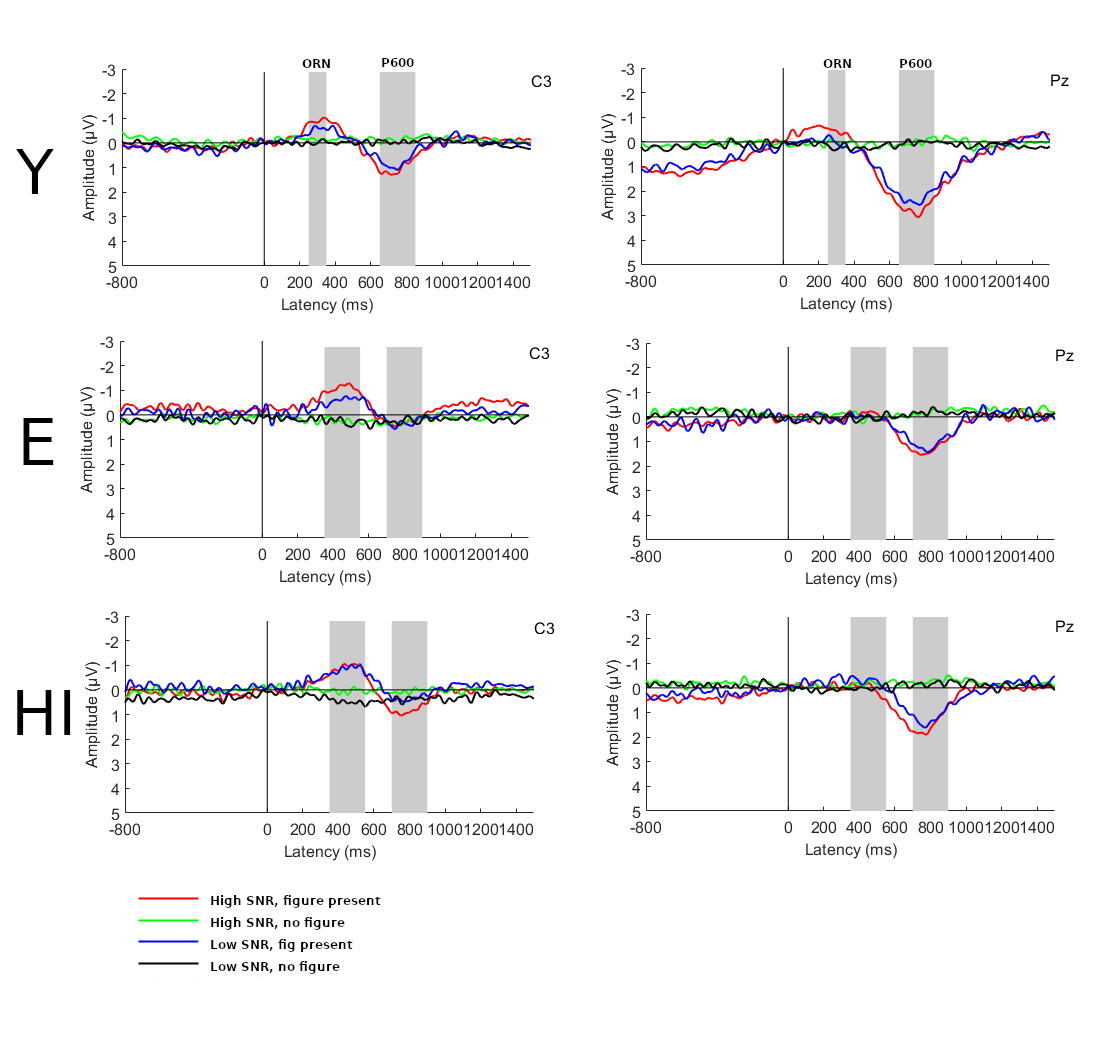
\includegraphics[width=0.6\linewidth]{erps2_legend}
	\captionof{figure}{\color{Green} ORN and P600 event-related potentials (respective time windows marked in grey) on the C3 and Pz electrodes for each group: Y = young, E = elderly with normal hearing, HI = hearing impaired elderly}
\end{center}\vspace{0cm}

%----------------------------------------------------------------------------------------
%	CONCLUSIONS
%----------------------------------------------------------------------------------------

\section*{Conclusions}

The preliminary data obtained in this study corroborates the hypothesis that the aging related impairment of auditory object detection in noise is partly due to changes in brain functionality which are independent of hearing impairment and can also be observed when hearing thresholds are within the normal range. Specifying this conclusion, the ERP results suggest that the age related listening impairments in listening under noisy conditions mainly stem from later stages of sound processing while early, low-level object detection mechanisms remain intact. Given the high level of neural plasticity still present even in the aging brain \autocite{Grady2012}, information about impaired neural processes which are independent of peripheral deterioration opens future possibilities of developing new training programs. In addition to better hearing, such trainings could improve the quality of life of the elderly, by increasing their sense of security, reducing social isolation and the risk of dementia \autocite{Slade2020}.

\section*{Future Research}

Functional connectivity analysis will complement our current findings with further data that might prove informative with regards to the exact neural processes involved. Furthermore, a subsequent study will address the question of whether figure-ground segregation training can improve the ability to listen in noisy environments in the elderly.

 %----------------------------------------------------------------------------------------
%	REFERENCES
%----------------------------------------------------------------------------------------
\vspace{100pt}
\subsection*{References}
\AtNextBibliography{\tiny}
\printbibliography[heading=none]

%----------------------------------------------------------------------------------------
%	ACKNOWLEDGEMENTS
%----------------------------------------------------------------------------------------

\subsection*{Acknowledgements}
\tiny
This research project was supported by grant nr. 123790 of the Hungarian Scientific Research Fund (OTKA) and the Bolyai Foundation (PI: Brigitta Tóth).

%----------------------------------------------------------------------------------------

\end{multicols}
\end{document}